\Chapter{STABILITE DYNAMIQUE DU MOUVEMENT DE ROTATION D'UNE ROUE CYR}\label{sec:Theme2}

\section{Etude théorique}
\subsection{Description du mouvement}
On étudie ici le second mouvement caractéristique de la roue Cyr, analogue au mouvement du disque d'Euler. Le mouvement se découpe en deux phases, une première phase au cours de laquelle la roue décrit des cercles en roulant sur sa tranche, puis une deuxième phase où elle oscille en tournant de plus en plus vite avant de tomber à plat, stoppant net le mouvement. Ces deux phases correspondent à l'énchainement de deux figures de roue Cyr, la "roue" pour la phase 1 et la pièce pour la phase 2. \\
Ce qui suit est basé sur l'article de Batista \cite{Batista}, dont la démarche et le modèle mathématique développés pour le disque d'Euler ont été adaptés à la géométrie torique de la roue Cyr. De même que Batista, l'objectif est de développer des cartes de stabilité dynamiques, avec d'autres variables adaptées à notre cas.

\subsection{Hypothèses}
\begin{itemize}
    \item On se place en régime stationnaire: les variables qui prennent ainsi des valeurs constantes seront indicées d'un 0.
    \item On considère que la roue évolue sur un sol rugueux: il n'y a pas de glissement au niveau du point de contact.
    \item Le mouvement est étudié pour des valeurs de $\theta_0$ strictement comprises entre 0 et $\pi/2$ radians.
\end{itemize}

\subsection{Mise en équations}
\subsubsection{Variables et systèmes de coordonnées}

\begin{table}[htbp]
  \centering
  \caption{Constantes et variables des modèle analytiques}
  \begin{tabular}{|c|l|}
    \hline\rowcolor[gray]{0.8}\color{black}
    Symbole         & Description\\\hline
    
    $A$             & Point autour duquel la roue roule en dessinant des cercles\\
    $C$             & Centre de gravité de la roue\\
    $(F_x,F_y,F_z)$          & Composante de la force de réaction au point $P$ dans $C_{xzy}$ \\
    $(M_x,M_y,M_z)$          & Composante du moment de réaction au point $P$ dans $C_{xzy}$ \\
    $P$             & Point de contact entre la roue et le sol\\
    $R$             & Rayon médian de la roue\\
    $r_c$             & Rayon des cercles dessinés par la roue, obtenus par\\
    & projection du centre de masse au sol\\
    $(v_{Cx0},v_{Cy0},v_{Cz0})$           & Composantes de la vitesse du point C dans $C_{xzy}$ en régime permanent \\
    $(X_C,Y_C,Z_C)$           & Position du centre de gravité dans le reférentiel $OXYZ$\\
    $(\psi,\theta,\phi)$       & Position angulaire de la roue dans $OXYZ$\\
    
    $\Omega_0$          & Vitesse angulaire par rapport à l'axe Z en régime permanent\\
    $(\omega_{10},\omega_{20},\omega_{30})$          & Composantes de la vitesse angulaire $\vec{omega_0}$ dans $C{\xi \eta \zeta}$ en régime permanent\\\hline
    
    
  \end{tabular}
  \label{tab:batista}
\end{table}

On reprend les trois référentiels utilisés par Batista, schématisés en figures \ref{fig:ref1} et \ref{fig:ref2}: le référentiel fixe  $OXYZ$, et les référentiels mobiles $C_{xzy}$ et $C_{\xi\eta\zeta}$ ayant pour origine le centre de gravité de la roue. $C_{xzy}$ est décalé de $OXYZ$ par une rotation d'angle $\psi$ autour de l'axe $Z$ et $C_{\xi\eta\zeta}$ est décalee de $C_{xzy}$ par une rotation d'angle $\theta$ autour de l'axe $x$.

\begin{figure}[htb]
\centering
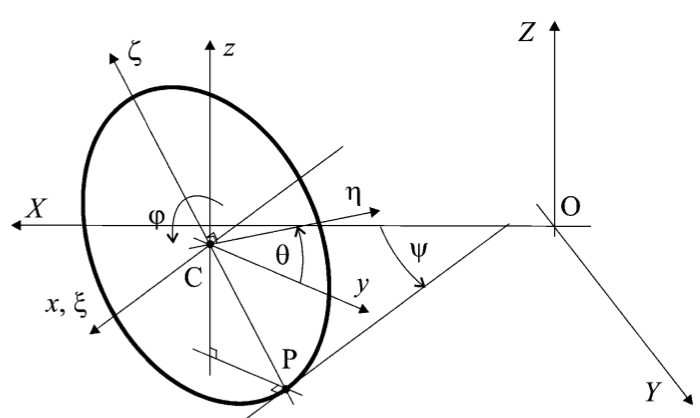
\includegraphics[width=4in]{batista/ref1.png}
\caption{Systèmes de coordonnées, tiré de l'article de Batista  \cite{Batista}. On utilise trois référentiels: un référentiel fixe, et deux référentiels liés à la roue, dont un correspond aux angles d'Euler.}
\label{fig:ref1}
\end{figure}

\begin{figure}[htb]
\centering
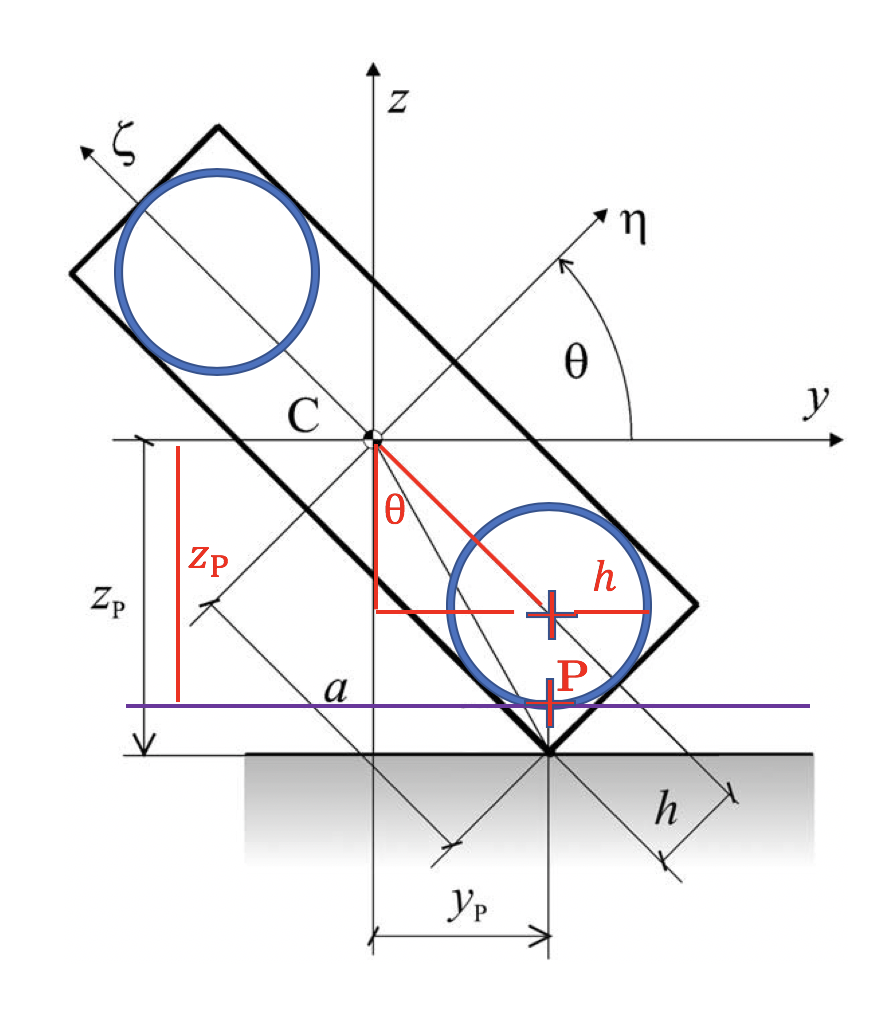
\includegraphics[width=3in]{batista/ref2.png}
\caption{Système de coordonnés, adapté de l'article de Batista \cite{Batista}. Nous étudions ici non pas un disque mais un tore, ce qui change, entre autres, l'expression de la position du point de contact $P$.}
\label{fig:ref2}
\end{figure}

\subsubsection{Equations}
On considère une roue à géométrie torique de rayon médian $R$ et de rayon externe de section $r_2$.\\
La position de la roue dans les référentiels présentés en figures \ref{fig:ref1} et \ref{fig:ref2} est décrite par les angles d'Euler: \\
$\theta$ décrit son inclinaison par rapport à la verticale: pour $\theta=\frac{\pi}{2}$, la roue est à plat sur le sol. \\
$\phi$ décrit la rotation de la roue, autour de son axe $\eta$, \\
$\psi$ décrit la rotation de la roue autour de l'axe $Z$ du référentiel fixe. \\

On se place en régime permanent: certaines des variables deviennent donc des constantes et seront indexées d'un zéro dans ce qui suit.
On note $(X_C,Y_C,Z_C)$ la position du centre de gravité dans le reférentiel $OXYZ$, $(v_{Cx0},v_{Cy0},v_{Cz0})$ les composantes de la vitesse du point C dans $C_{xzy}$, $(\omega_{10},\omega_{20},\omega_{30})$ les composantes de la vitesse angulaire $\vec{omega_0}$ dans $C{\xi \eta \zeta}$ et $\Omega$ la vitesse angulaire par rapport à l'axe $Z$.

Le mouvement de la roue est régie par les équations cinématiques suivantes \cite{Batista}:

 \begin{align} 
    \frac{dX_C}{dt} &=v_{Cx0} \cos{\psi}- v_{Cy0} \sin{\psi}  & \frac{d\psi}{dt}&=\Omega_0=\frac{\omega_{30}}{\cos{\theta_0}} \nonumber\\
    \frac{dY_C}{dt} &=v_{Cx0} \sin{\psi}- v_{Cy0} \cos{\psi} & \frac{d\theta}{dt}&=\omega_{10}=0 \nonumber\\
    \frac{dZ_C}{dt} &=v_{Cz0} & \frac{d\phi}{dt}&=\omega_{20}-\omega_{30} \tan{\theta_0}
    \label{eq:b1}
\end{align}



Les coordonnées du point de contact P dans C{xzy}, schématisé dans la figure \ref{fig:ref2} s'expriment:
\begin{align}
    x_P&=0 \nonumber\\
    y_P&=R\sin{\theta_0} \nonumber\\
    z_P&=-R\cos{\theta_0}-r_2
  \label{eq:b2}
\end{align}

D'après la règle de transport des torseurs, la vitesse du point de contact dans $C_{xzy}$ s'écrit:
\begin{equation}
    \vec{v_{P0}}=\vec{v_{C0}}+\vec{\omega_0} \wedge \vec{CP},
  \label{eq:b3}
\end{equation}

avec $\vec{\omega_0}=(\omega_{10},\omega_{20},\omega_{30})$
et $\vec{CP}=(0,R\sin{\theta_0},-R\cos{\theta_0}-r_2)$ .



Les composantes de la vitesse au point de contact dans $C_{xzy}$ s'écrivent donc:
\begin{align}
    v_{Px_0}&=v_{Cx_0}-\omega_{20} (R\cos{\theta_0}+r_2) -\omega_{30} R\sin{\theta} \nonumber \\
    v_{Py_0}&=v_{Cy_0} + \omega_{10} (R\cos{\theta_0}+r_2)= v_{Cy_0} \nonumber\\
    v_{Pz_0}&=v_{Cz_0} + \omega_{10} R\sin{\theta_0} = v_{Cz_0}
  \label{eq:b4}
\end{align}

On a fait l'hypothèse d'un sol rugueux: on a donc $v_{Px0}=v_{Py0}=0$, et comme le contact entre le sol et la roue est permanent, $v_{Pz0}=0=v_{Cz_0}$.


Les composantes de l'accélération du centre d'inertie de la roue dans $C{xzy}$ s'expriment à partir de l'équation \ref{eq:b1} projetée dans $C{xzy}$:

\begin{align}
    a_{Cx0}&=\frac{dv_{Cx0}}{dt}-\Omega_0 v_{Cy0}=-\Omega_0 v_{Cy0} \nonumber\\
    a_{Cy0}&=\frac{dv_{Cy0}}{dt} + \Omega_0 v_{Cx0}=\Omega_0 v_{Cx0}\nonumber\\
    a_{Cz0}&=\frac{dv_{Cz0}}{dt} = 0
  \label{eq:b5}
\end{align}

L'équation \ref{eq:b5} combinée à la relation fondamentale de la dynamique en translation donne:

\begin{align}
    m_r\Omega_0 v_{Cy0}&=-F_x \nonumber\\
    m_r \Omega_0 v_{Cx0}&=F_y \nonumber\\
    m_r(\frac{dv_{Cz0}}{dt})&=-mg+F_z=0,
  \label{eq:b7}
\end{align}

où $F_x$, $F_y$ et $F_z$ sont les composantes de la force de réaction $\mathbf{F}$ au point P, exprimées dans $C_{xyz}$.

Le moment cinétique au centre de masse s'exprime $\vec{L_{C0}}=I \cdot \vec{\omega}$, avec pour tenseur d'inertie:
\begin{equation}
    I=
\begin{pmatrix}
   m_r (\frac{1}{2}R^2+\frac{5}{8}r_2^2) & 0  &  0 \\
  0 &  m_r(R^2+\frac{3}{4}r_2^2) & 0 \\
  0 & 0 & m_r (\frac{1}{2}R^2+\frac{5}{8}r_2^2)
\end{pmatrix}
\label{eq:inertie}
\end{equation}


Notons $k_1^2=\frac{1}{2}R^2+\frac{5}{8}r_2^2$ et $k_2^2=R^2+\frac{3}{4}r_2^2$

Les composantes du moment cinétique en $C$ dans $C_{\xi \eta \zeta}$ s'écrivent donc:
\begin{align}
    L_{C\xi0 }&=m_r k_1^2 \omega_{10}=0 \nonumber\\
    L_{C\eta0}&=m_r k_2^2 \omega_{20} \nonumber\\
    L_{C\zeta0 }&=m_r k_1^2 \omega_{30}
  \label{eq:b6}
\end{align}

La relation fondamentale de la dynamique en rotation appliquée au centre de masse de la roue dans le référentiel $C_{xyz}$ donne:

\begin{equation}
    \frac{d \mathbf{L_{C0}}}{dt} + \mathbf{R} \wedge \mathbf{L_{C0}} = \mathbf{M}+ \overrightarrow{CP} \wedge \mathbf{F} 
\label{eq:rfdr}
\end{equation}

où $\mathbf{R}$ est la vitesse angulaire de $C_{\xi \eta \zeta}$ et $\mathbf{M}$ est le moment de réaction au point P exprimé dans $C_{xyz}$, de composantes $M_x$, $M_y$ et $M_z$.

Le référentiel $C_{\xi \eta \zeta}$ a été défini de telle sorte que sa vitesse angulaire $\mathbf{R}$ est égale à la vitesse angulaire $\mathbf{\omega}$ de la roue sans la rotation en $\phi$ autour de l'axe $\eta$.

On a donc
\begin{equation}
   \mathbf{R}= \begin{pmatrix}
    \omega_1  \\
    \omega_2 - \frac{d\phi}{dt} \\
    \omega_3     
\end{pmatrix} 
=
\begin{pmatrix}
    \omega_1  \\
    \omega_{3}\tan(\theta) \\
    \omega_3     
\end{pmatrix} 
\label{eq:rb}
\end{equation}

En régime permanent, \ref{eq:rb} devient:

\begin{equation}
   \mathbf{R}= \begin{pmatrix}
    0  \\
    \omega_{30}\tan(\theta_0) \\
    \omega_{30}     
\end{pmatrix} 
\label{eq:rb2}
\end{equation}

En substituant \ref{eq:b6} et \ref{eq:rb2} dans \ref{eq:rfdr}, on obtient:

\begin{align}
    m_r(k_2^2\omega_{20}-k_1^2\omega_{30} \tan{\theta_0})\omega_{30} +(R\cos{\theta_0}+r_2)F_y + R\sin{\theta_0}F_z + M_x &=0 \nonumber\\
    -(R+r_2)F_x + M_y \cos{\theta_0} +M_z \sin{\theta_0}&=0 \nonumber\\
    m_r(-k_2^2\omega_{20}+k_1^2\omega_{30} \tan{\theta_0})\omega_{10} + hF_x - M_y \sin{\theta_0} +M_z \cos{\theta_0}&=0
  \label{eq:b8}
\end{align}

La dérivée de l'énergie mécanique s'exprime: 
\begin{equation}
    \frac{dE}{dt}=P_F + P_M, 
    \label{eq:be1}
\end{equation}

avec $P_F$ et $P_M$, les puissances de la fore de réaction $F$ et du moment de réaction $M$, ce qui donne:

\begin{equation}
    \frac{dE}{dt}=\vec{v_P} \cdot \vec{F} + \vec{\omega} \cdot \vec{M}
    \label{eq:be2}
\end{equation}

En régime stationnaire, on a $\dfrac{dE}{dt}=0$, et comme on a fait l'hypothèse du sol rugueux, $\vec{v_P}=\vec{0}$, \ref{eq:be2} devient donc: $$\vec{\omega} \cdot \vec{M}$$

Le disque doit avoir une vitesse de rotation pour qu'il y ait un mouvement à étudier, on en déduit donc $\vec{M}=\vec{0}$

Les équations \ref{eq:b7} et \ref{eq:b8} deviennent alors:

\begin{align}
    &F_y=m_r \Omega_0 v_{Cx0} \nonumber\\
    &m_r(k_2^2\omega_{20}-k_1^2\omega_{30} \tan{\theta_0})\omega_{30} +(R\cos{\theta_0}+r_2)m_r \Omega_0 v_{Cx0} + R\sin{\theta_0}mg =0
  \label{eq:b9}
\end{align}

Or, on sait de l'équation \ref{eq:b1} que:

\begin{align}
    \omega_{20}&=\omega_0 + \Omega_0 \sin{\theta_0} \nonumber\\
    \omega_{30}&=\Omega_0 \cos{\theta_0},
  \label{eq:b10}
\end{align}

et de l'équation \ref{eq:b2} que:

\begin{equation}
    v_{Cx0}=(R+r_2)\omega_{20}-r_2\omega_{30}
    \label{eq:b10b}
\end{equation}

En substituant \ref{eq:b10} et \ref{eq:b11} dans \ref{eq:b9}, on obtient:

\begin{align}
     &m_r(k_2^2(\omega_0 + \Omega_0 \sin{\theta_0})-k_1^2(\Omega_0 \cos{\theta_0}) \tan{\theta_0})(\Omega_0 \cos{\theta_0})  \nonumber\\
    &+(R\cos{\theta_0}+r_2)m_r \Omega_0 ((R+r_2)(\omega_0 + \Omega_0 \sin{\theta_0})-r_2\Omega_0 \cos{\theta_0}) + R\sin{\theta_0}m_r g =0
  \label{eq:b11}
\end{align}

soit

\begin{align}
     &[(k_2^2-k_1^2)\sin(\theta_0)\cos(\theta_0)+(R \cos(\theta_0)+r_2)[(R+r_2)\sin(\theta_0)-r_2 \cos(\theta_0)]]\Omega_0^2 \nonumber\\
     &+\omega_0[k_2^2 \cos(\theta_0)+(R+r_2)(R \cos(\theta_0))] \Omega_0 + R g \sin(\theta_0) =0
  \label{eq:b12}
\end{align}

On définit la longueur adimensionnelle $$\hat{L}=\dfrac{\sqrt{(k_2^2-k_1^2)\sin(\theta_0)\cos(\theta_0)+(R \cos(\theta_0)+r_2)[(R+r_2)\sin(\theta_0)-r_2 \cos(\theta_0)]}}{R\sin{\theta_0}}$$,
et la pulsation adimensionnelle $\hat{\omega_0}=\omega_0 \sqrt{\dfrac{R+r_2}{g}}$.

Ecrit sous forme adimensionnelle, \ref{eq:b12} devient:

\begin{equation}
 \begin{split}
     \frac{R \sin(\theta_0)\hat{L}^2}{g} \Omega_0^2+\hat{\omega_0} \frac{k_2^2+R(R+r_2)}{R \tan(\theta_0) \sqrt{g(R+r_2)}} \Omega_0+1 =0
 \end{split}
  \label{eq:b12a}
\end{equation}

L'équation \ref{eq:b11} se traduit ainsi: pour que le régime stationnaire puisse exister, l'équation polynomiale en $\Omega_0$ doit avoir une solution réelle. L'existence de cette solution dépend des valeurs de $(\theta_0,\omega_0)$. On peut ainsi tracer une première partie de la carte de stabilité, en séparant graphiquement les cas où le régime stationnaire est possible, et les cas où il ne peut pas exister.

\begin{equation}
 \Omega_0=g \frac{\hat{\omega_0} \frac{k_2^2+R(R+r_2)}{R \tan(\theta_0) \sqrt{g(R+r_2)}}\pm \sqrt{\Delta}}{2R\sin(\theta_0)\hat{L}^2},
  \label{eq:b13}
\end{equation}

avec 

\begin{equation}
 \Delta=(\hat{\omega_0} \frac{k_2^2+R(R+r_2)}{R \tan(\theta_0) \sqrt{g(R+r_2)}})^2-4\frac{ \hat{L}^2 R \sin(\theta_0)}{g}
  \label{eq:b14}
\end{equation}

Pour que $\Omega_0$ soit réel, il faut $\Delta \geq 0$
Lorsque $\Delta < 0$ l'équilibre n'existe pas

La frontière de l'équilibre dynamique est décrite par l'équation:

\begin{equation}
(\hat{\omega_0} \frac{k_2^2+R(R+r_2)}{R \tan(\theta_0) \sqrt{g(R+r_2)}})^2-4\frac{ \hat{L}^2 R \sin(\theta_0)}{g} = 0
\label{eq:b15}
\end{equation}

Ce qui équivaut à:

\begin{equation}
 \hat{\omega_0}= \pm \frac{2\hat{L} R \tan(\theta_0) \sqrt{R(R+r_2)\sin(\theta_0)}}{k_2^2+R(R+r_2)}
  \label{eq:b16}
\end{equation}

Lorsque $$ |\hat{\omega_0}| < \frac{2\hat{L} R \tan(\theta_0) \sqrt{R(R+r_2)\sin(\theta_0)}}{k_2^2+R(R+r_2)},
$$
 la force centrifuge et la réaction du sol ne peuvent plus contrebalancer l'effet de la gravité.
 
\begin{figure}[h]
\centering
\def\svgwidth{370}
%% Creator: Inkscape inkscape 0.92.2, www.inkscape.org
%% PDF/EPS/PS + LaTeX output extension by Johan Engelen, 2010
%% Accompanies image file 'bat12.eps' (pdf, eps, ps)
%%
%% To include the image in your LaTeX document, write
%%   \input{<filename>.pdf_tex}
%%  instead of
%%   \includegraphics{<filename>.pdf}
%% To scale the image, write
%%   \def\svgwidth{<desired width>}
%%   \input{<filename>.pdf_tex}
%%  instead of
%%   \includegraphics[width=<desired width>]{<filename>.pdf}
%%
%% Images with a different path to the parent latex file can
%% be accessed with the `import' package (which may need to be
%% installed) using
%%   \usepackage{import}
%% in the preamble, and then including the image with
%%   \import{<path to file>}{<filename>.pdf_tex}
%% Alternatively, one can specify
%%   \graphicspath{{<path to file>/}}
%% 
%% For more information, please see info/svg-inkscape on CTAN:
%%   http://tug.ctan.org/tex-archive/info/svg-inkscape
%%


\begingroup%
  \makeatletter%
  \providecommand\color[2][]{%
    \errmessage{(Inkscape) Color is used for the text in Inkscape, but the package 'color.sty' is not loaded}%
    \renewcommand\color[2][]{}%
  }%
  \providecommand\transparent[1]{%
    \errmessage{(Inkscape) Transparency is used (non-zero) for the text in Inkscape, but the package 'transparent.sty' is not loaded}%
    \renewcommand\transparent[1]{}%
  }%
  \providecommand\rotatebox[2]{#2}%
  \ifx\svgwidth\undefined%
    \setlength{\unitlength}{432bp}%
    \ifx\svgscale\undefined%
      \relax%
    \else%
      \setlength{\unitlength}{\unitlength * \real{\svgscale}}%
    \fi%
  \else%
    \setlength{\unitlength}{\svgwidth}%
  \fi%
  \global\let\svgwidth\undefined%
  \global\let\svgscale\undefined%
  \makeatother%
  \begin{picture}(1,0.83333333)%
    \put(0,0){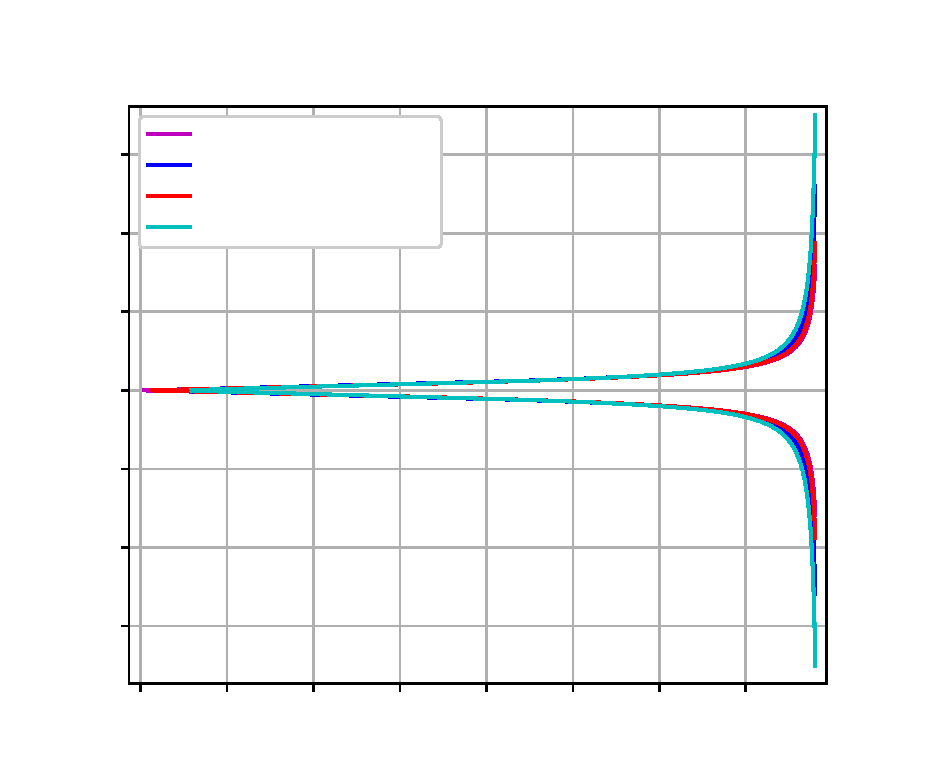
\includegraphics[width=\unitlength]{imagesbat/bat12.eps}}%
    \put(0.11923819,0.05788495){\color[rgb]{0,0,0}\makebox(0,0)[lb]{\smash{0.0}}}%
    \put(0.21531203,0.05788495){\color[rgb]{0,0,0}\makebox(0,0)[lb]{\smash{0.2}}}%
    \put(0.31138425,0.05788495){\color[rgb]{0,0,0}\makebox(0,0)[lb]{\smash{0.4}}}%
    \put(0.40745832,0.05788495){\color[rgb]{0,0,0}\makebox(0,0)[lb]{\smash{0.6}}}%
    \put(0.50353008,0.05788495){\color[rgb]{0,0,0}\makebox(0,0)[lb]{\smash{0.8}}}%
    \put(0.59960415,0.05788495){\color[rgb]{0,0,0}\makebox(0,0)[lb]{\smash{1.0}}}%
    \put(0.69567822,0.05788495){\color[rgb]{0,0,0}\makebox(0,0)[lb]{\smash{1.2}}}%
    \put(0.79174998,0.05788495){\color[rgb]{0,0,0}\makebox(0,0)[lb]{\smash{1.4}}}%
    \put(0.05,0.14706226){\color[rgb]{0,0,0}\makebox(0,0)[lb]{\smash{$-30$}}}%
    \put(0.05,0.23435879){\color[rgb]{0,0,0}\makebox(0,0)[lb]{\smash{$-20$}}}%
    \put(0.05,0.3216574){\color[rgb]{0,0,0}\makebox(0,0)[lb]{\smash{$-10$}}}%
    \put(0.09407546,0.40895601){\color[rgb]{0,0,0}\makebox(0,0)[lb]{\smash{0}}}%
    \put(0.07935486,0.49625462){\color[rgb]{0,0,0}\makebox(0,0)[lb]{\smash{10}}}%
    \put(0.07935486,0.58355323){\color[rgb]{0,0,0}\makebox(0,0)[lb]{\smash{20}}}%
    \put(0.07935486,0.67084952){\color[rgb]{0,0,0}\makebox(0,0)[lb]{\smash{30}}}%
    \put(0.470353008,0.01){\color[rgb]{0,0,0}\makebox(0,0)[lb]{\smash{ $\theta_0 (rad)$}}}%
    \put(0.04524745,0.4){\color[rgb]{0,0,0}\rotatebox{90}{\makebox(0,0)[lb]{\smash{$\hat{\omega_0} $}}}}%
    \put(0.21064814,0.69492128){\color[rgb]{0,0,0}\makebox(0,0)[lb]{\smash{\footnotesize $R=1.0 m, r_2=1.0 cm$}}}%
    \put(0.21064814,0.66030785){\color[rgb]{0,0,0}\makebox(0,0)[lb]{\smash{\footnotesize $R=1.0 m, r_2=5.0 cm$}}}%
    \put(0.21064814,0.62569443){\color[rgb]{0,0,0}\makebox(0,0)[lb]{\smash{\footnotesize $R=0.5 m, r_2=1.0 cm$}}}%
    \put(0.21064814,0.591081){\color[rgb]{0,0,0}\makebox(0,0)[lb]{\smash{\footnotesize $R=0.5 m, r_2=5.0 cm$}}}%
    \put(0.59960415,0.23435879){\color[rgb]{0,0,0}\makebox(0,0)[lb]{\smash{stable}}}%
    \put(0.59960415,0.58355323){\color[rgb]{0,0,0}\makebox(0,0)[lb]{\smash{stable}}}%
    \put(0.75,0.40895601){\color[rgb]{0,0,0}\makebox(0,0)[lb]{\smash{instable}}}%
  \end{picture}%
\endgroup%

\caption{Première partie de la carte de stabilité. La frontière détermine l'existence d'une position d'équilibre dynamique pour chaque couple ($\theta_0,\hat{\omega_0}$), où $\hat{\omega_0}$ correspond à la vitesse de rotation adimensionnelle, $\hat{\omega_0}=\omega_0 \sqrt{\dfrac{R+r_2}{g}}$}
\end{figure}

\section{Réponse à une perturbation}

On étudie à présent la réponse du système en régime permanent à une petite perturbation, ce qui se traduit par l'ajout d'un terme de pulsation $\sigma$ aux variables $\theta, \omega_1, \omega_2, \omega_3$: \\


\begin{align}
 \theta&=\theta_0 + \epsilon \Tilde{\theta} e^{i \sigma t} \nonumber\\
 \omega_1&= \omega_{10} + \epsilon \Tilde{\omega_1} e^{i \sigma t} = \epsilon \Tilde{\omega_1} e^{i \sigma t} = \frac{d\theta }{dt} \nonumber\\
 \omega_2&= \omega_{20} + \epsilon \Tilde{\omega_2} e^{i \sigma t} \nonumber\\
 \omega_3&= \omega_{30} + \epsilon \Tilde{\omega_3} e^{i \sigma t}
  \label{eq:b17}
\end{align}

Avec les variables \ref{eq:b17}, les coordonnées du point de contact P dans C{xzy}, schématisé dans la figure \ref{fig:ref2} s'expriment à présent:
\begin{align}
    x_P&=0 \nonumber\\
    y_P&=R\sin{\theta} \nonumber\\
    z_P&=-R\cos{\theta}-r_2.
  \label{eq:b2p}
\end{align}

Et les composantes de la vitesse angulaire deviennent:

\begin{equation}
    \vec{\omega}=(\omega_1,\omega_2,\omega_3)
    \label{eq:b3p}
\end{equation}

En substituant \ref{eq:b2p} et \ref{eq:b3p} dans \ref{eq:b3}, et en conservant l'hypothèse d'un sol parfaitement rugueux ($\vec{v_P}=\vec{0}$) on obtient la nouvelle expression des composantes de la vitesse du centre de gravité dans $C_{xzy}$:

\begin{align}
    v_{Cx}&=(R\cos(\theta)+r_2)\omega_2+R \sin(\theta)\omega_3 \nonumber\\
    v_{Cy} &= -(R\cos(\theta)+r_2)\omega_1 \nonumber\\
    v_{Cz} &= -R \sin(\theta)\omega_1
  \label{eq:b18}
\end{align}

En simplifiant \ref{eq:b18} avec les développements limités \ref{eq:bdl}, en ne gardant que les termes d'ordre 1 en $\epsilon$, on obtient \ref{eq:b18b}:

\begin{align}
    \cos(\theta_0 + \epsilon \Tilde{\theta} e^{i \sigma t})&=\cos(\theta_0)- \sin(\theta_0)\epsilon \Tilde{\theta} e^{i \sigma t} + o(\epsilon) \nonumber\\
    \sin(\theta_0 + \epsilon \Tilde{\theta} e^{i \sigma t})&=\sin(\theta_0)+ \cos(\theta_0)\epsilon \Tilde{\theta} e^{i \sigma t} + o(\epsilon)\nonumber\\
    \tan(\theta_0 + \epsilon \Tilde{\theta} e^{i \sigma t})&=\tan(\theta_0)+ (1+\tan(\theta_0)^2)\epsilon \Tilde{\theta} e^{i \sigma t} + o(\epsilon)
\label{eq:bdl}
\end{align}

\begin{align}
    v_{Cx}=&(R\cos(\theta_0)+r_2)\omega_{20}+R \sin{\theta_0}\omega_{30} \nonumber\\ 
    &+ \epsilon e^{i \sigma t}[(R\cos(\theta_0)+r_2) \Tilde{\omega_2} +R(\omega_{30}\cos(\theta_0)-\sin(\theta_0)\omega_{20}) \Tilde{\theta}+R\sin(\theta_0) \Tilde{\omega_3} ] \nonumber\\ 
    v_{Cy} =& -(R\cos(\theta_0)+r_2)\epsilon \Tilde{\omega_1} e^{i \sigma t} \nonumber\\ 
    v_{Cz} =& -R \sin(\theta_0)\epsilon \Tilde{\omega_1} e^{i \sigma t}
  \label{eq:b18b}
\end{align}

Les composantes de l'accélération du centre d'inertie de la roue dans $C{xzy}$ s'expriment à partir de l'équation \ref{eq:b1} projetée dans $C{xzy}$:

\begin{align}
    a_{Cx}&=\frac{dv_{Cx}}{dt}-\Omega v_{Cy} \nonumber\\
    a_{Cy}&=\frac{dv_{Cy}}{dt} + \Omega v_{Cx}\nonumber\\
    a_{Cz}&=\frac{dv_{Cz}}{dt} 
  \label{eq:b19b}
\end{align}
\\
L'équation \ref{eq:b1}, permet d'exprimer $\Omega$:
\begin{equation}
    \Omega=\frac{\omega_{30}}{\cos{\theta_0}} + (\frac{\tilde{\omega_3}}{\cos(\theta_0)}+\frac{\sin(\theta_0)}{\cos(\theta_0)^2}\omega_{30}\tilde{\theta})\epsilon e^{i \sigma t}
    \label{eq:Omega}
\end{equation}


En substituant \ref{eq:b18b} à l'intérieur de \ref{eq:b19b}, on obtient:

\begin{align}
    a_{Cx}=& i \sigma \epsilon e^{i \sigma t}[(R\cos(\theta_0)+r_2) \Tilde{\omega_2} +R(\omega_{30}\cos(\theta_0)-\sin(\theta_0)\omega_{20}) \Tilde{\theta}+R\sin(\theta_0) \Tilde{\omega_3} ] \nonumber\\
    &+\Omega (R\cos(\theta_0)+r_2)\epsilon \Tilde{\omega_1} e^{i \sigma t} \nonumber\\
    a_{Cy}=& -i \sigma( R\cos(\theta_0)+r_2)\epsilon \Tilde{\omega_1} e^{i \sigma t} 
    + \Omega [(R\cos(\theta_0)+r_2)\omega_{20}+R \sin{\theta_0}\omega_{30} \nonumber\\ 
    &+ \epsilon e^{i \sigma t}[(R\cos(\theta_0)+r_2) \Tilde{\omega_2} +R(\omega_{30}\cos(\theta_0)-\sin(\theta_0)\omega_{20}) \Tilde{\theta}+R\sin(\theta_0) \Tilde{\omega_3} ] ]\nonumber \\
    a_{Cz}=& -i \sigma R \sin(\theta_0)\epsilon \Tilde{\omega_1} e^{i \sigma t} 
  \label{eq:b19b2}
\end{align}

D'après \ref{eq:b19b2} et la relation fondamentale de la dynamique en translation:

\begin{align}
  i \sigma \epsilon e^{i \sigma t}[(R\cos(\theta_0)+r_2) \Tilde{\omega_2} +R(\omega_{30}\cos(\theta_0)-\sin(\theta_0)\omega_{20}) \Tilde{\theta}+R\sin(\theta_0) \Tilde{\omega_3} ]& \nonumber \\
    +\Omega (R\cos(\theta_0)+r_2)\epsilon \Tilde{\omega_1} e^{i \sigma t}&=\frac{F_x}{m_r} \nonumber \\
    -i \sigma( R\cos(\theta_0)+r_2)\epsilon \Tilde{\omega_1} e^{i \sigma t}
    + \Omega [(R\cos(\theta_0)+r_2)\omega_{20}+R \sin{\theta_0}\omega_{30}& \nonumber\\ 
    + \epsilon e^{i \sigma t}[(R\cos(\theta_0)+r_2) \Tilde{\omega_2} +R(\omega_{30}\cos(\theta_0)-\sin(\theta_0)\omega_{20}) \Tilde{\theta}+R\sin(\theta_0) \Tilde{\omega_3} ] ]&=\frac{F_y}{m_r} \nonumber \\
    -i \sigma R \sin(\theta_0)\epsilon \Tilde{\omega_1} e^{i \sigma t}&=- g +\frac{F_z}{m_r}
  \label{eq:b20}
\end{align}

Le moment cinétique au centre de masse s'exprime $\vec{L_{C}}=I \cdot \vec{\omega}$, le tenseur d'inertie étant donné en \ref{eq:inertie}.

Les composantes du moment cinétique dans $C_{\xi \eta \zeta}$ s'écrivent donc:
\begin{align}
    L_{C\xi }&=m_r k_1^2 \omega_{1} \nonumber\\
    L_{C\eta}&=m_r k_2^2 \omega_{2} \nonumber\\
    L_{C\zeta }&=m_r k_1^2 \omega_{3}
  \label{eq:b6b}
\end{align}

La relation fondamentale de la dynamique en rotation appliquée au centre de masse de la roue dans le référentiel $C_{xyz}$ donne:

\begin{equation}
    \frac{d \mathbf{L_{C}}}{dt} + \mathbf{R} \wedge \mathbf{L_{C}} = \mathbf{M}+ \overrightarrow{CP} \wedge \mathbf{F} 
\label{eq:rfdr2}
\end{equation}

où $\mathbf{R}$ est la vitesse angulaire de $C_{\xi \eta \zeta}$ et $\mathbf{M}$ est le moment de réaction au point P exprimé dans $C_{xyz}$, de composantes $M_x$, $M_y$ et $M_z$.

L'expression de $\mathbf{R}$ a été déterminée en \ref{eq:rb}

\begin{equation}
   \mathbf{R}= 
\begin{pmatrix}
    \omega_1  \\
    \omega_{3}\tan(\theta) \\
    \omega_3     
\end{pmatrix} 
\label{eq:rb3}
\end{equation}

En substituant \ref{eq:b6b} et \ref{eq:rb3} dans \ref{eq:rfdr2}, on obtient:

\begin{align}
    k_1^2\frac{d\omega_1}{dt} &=(k_2^2\omega_2-k_1^2\omega_3 \tan{\theta})\omega_3+(R\cos{\theta}+r_2)\frac{F_y}{m_r}+ R\sin{\theta}\frac{F_z}{m_r} \nonumber \\
    k_2^2\frac{d\omega_2}{dt} &=-(R+r_2) \frac{F_x}{m_r} \nonumber \\
    k_1^2\frac{d\omega_3}{dt} &=(-k_2^2\omega_2+k_1^2\omega_3 \tan(\theta))\omega_1 + r_2 \frac{F_x}{m_r}
  \label{eq:b21}
\end{align}

On substitue \ref{eq:b17} dans \ref{eq:b21}, en simplifiant les expressions à l'aide de développements limités et on néglige les termes de perturbation d'ordre supérieur ou égal à 2.

\begin{align}
    k_1^2 i \sigma\epsilon \Tilde{\omega_1} e^{i \sigma t} =&(k_2^2\omega_{20}-k_1^2\omega_{30} \tan{\theta_0})\omega_{30}+\epsilon e^{i\sigma t}[k_2^2 \omega_{20} \tilde{\omega_3}+k_2^2 \omega_{30} \tilde{\omega_2} -2k_1^2\omega_{30} \tan(\theta_0)\tilde{\omega_3} \nonumber\\
    &-k_1^2 \omega_{30}^2(1+\tan(\theta_0)^2)\tilde{\theta} ]+(R(\cos(\theta_0)- \sin(\theta_0)\epsilon \Tilde{\theta} e^{i \sigma t})+r_2)\frac{F_y}{m_r}\nonumber \\
    &+ R(\sin(\theta_0)+ \cos(\theta_0)\epsilon \Tilde{\theta} e^{i \sigma t})\frac{F_z}{m_r} \nonumber\\ 
    k_2^2 i \sigma\epsilon \Tilde{\omega_2} e^{i \sigma t}=&-(R+r_2) \frac{F_x}{m_r} \nonumber\\ 
    k_1^2 i \sigma\epsilon \Tilde{\omega_3} e^{i \sigma t}=&(-k_2^2\omega_{20}+k_1^2\omega_{30} \tan(\theta_0))\epsilon \Tilde{\omega_1} e^{i \sigma t} + r_2 \frac{F_x}{m_r}
  \label{eq:b22}
\end{align}

On substitue ensuite \ref{eq:b20} et \ref{eq:Omega} dans \ref{eq:b22} 

\begin{align}
    k_1^2 i \sigma \epsilon \Tilde{\omega_1} e^{i \sigma t} =&(k_2^2\omega_{20}-k_1^2\omega_{30} \tan{\theta_0})\omega_{30}+\epsilon e^{i\sigma t}[k_2^2 \omega_{20} \tilde{\omega_3}+k_2^2 \omega_{30} \tilde{\omega_2} -2k_1^2\omega_{30} \tan(\theta_0)\tilde{\omega_3}\nonumber\\
    &-k_1^2 \omega_{30}^2(1+\tan(\theta_0)^2)\tilde{\theta} ]+(R(\cos(\theta_0)- \sin(\theta_0)\epsilon \Tilde{\theta} e^{i \sigma t})+r_2)[-i \sigma( R\cos(\theta_0)+r_2)\epsilon \Tilde{\omega_1} e^{i \sigma t} \nonumber\\
    &+ (\frac{\omega_{30}}{\cos{\theta_0}} + (\frac{\tilde{\omega_3}}{\cos(\theta_0)}+\frac{\sin(\theta_0)}{\cos(\theta_0)^2}\omega_{30}\tilde{\theta})\epsilon e^{i \sigma t}) [(R\cos(\theta_0)+r_2)\omega_{20}+R \sin{\theta_0}\omega_{30} \nonumber\\ 
    &+ \epsilon e^{i \sigma t}[(R\cos(\theta_0)+r_2) \Tilde{\omega_2} +R(\omega_{30}\cos(\theta_0)-\sin(\theta_0)\omega_{20}) \Tilde{\theta}+R\sin(\theta_0) \Tilde{\omega_3} ] ]] \nonumber\\
    &+ R(\sin(\theta_0)+ \cos(\theta_0)\epsilon \Tilde{\theta} e^{i \sigma t})[g-i \sigma R \sin(\theta_0)\epsilon \Tilde{\omega_1} e^{i \sigma t}] \nonumber\\
    k_2^2 i \sigma\epsilon \Tilde{\omega_2} e^{i \sigma t}=&-(R+r_2) [i \sigma \epsilon e^{i \sigma t}[(R\cos(\theta_0)+r_2) \Tilde{\omega_2} +R(\omega_{30}\cos(\theta_0)-\sin(\theta_0)\omega_{20}) \Tilde{\theta}+R\sin(\theta_0) \Tilde{\omega_3} ] \nonumber\\
    &+\frac{\omega_{30}}{\cos{\theta_0}} (R\cos(\theta_0)+r_2)\epsilon \Tilde{\omega_1} e^{i \sigma t}] \nonumber\\
    k_1^2 i \sigma\epsilon \Tilde{\omega_3} e^{i \sigma t}=&(-k_2^2\omega_{20}+k_1^2\omega_{30} \tan(\theta_0))\epsilon \Tilde{\omega_1} e^{i \sigma t} + r_2 [i \sigma \epsilon e^{i \sigma t}[(R\cos(\theta_0)+r_2) \Tilde{\omega_2} \nonumber\\
    &+R(\omega_{30}\cos(\theta_0)-\sin(\theta_0)\omega_{20}) \Tilde{\theta}+R\sin(\theta_0) \Tilde{\omega_3} ] 
    +\frac{\omega_{30}}{\cos{\theta_0}} (R\cos(\theta_0)+r_2)\epsilon \Tilde{\omega_1} e^{i \sigma t}]
\label{eq:b23}
\end{align}


En regroupant les termes \ref{eq:b23} devient:

\begin{align}
    \epsilon e^{i \sigma t} [k_2^2 \omega_{20} \tilde{\omega_3}+k_2^2 \omega_{30} \tilde{\omega_2} -2k_1^2\omega_{30} \tan(\theta_0)\tilde{\omega_3}
    -k_1^2 \omega_{30}^2(1+\tan(\theta_0)^2)\tilde{\theta} -k_1^2 i \sigma \Tilde{\omega_1} &\nonumber\\
    +(R\cos{\theta_0}+r_2)(-i \sigma( R\cos(\theta_0)+r_2) \Tilde{\omega_1}& \nonumber \\
    +\frac{\omega_{30}}{\cos{\theta_0}} [(R\cos(\theta_0)+r_2) \Tilde{\omega_2} 
    +R(\omega_{30}\cos(\theta_0)-\sin(\theta_0)\omega_{20}) \Tilde{\theta}
    +R\sin(\theta_0) \Tilde{\omega_3} ] & \nonumber \\
    + (\frac{\tilde{\omega_3}}{\cos(\theta_0)}+\frac{\sin(\theta_0)}{\cos(\theta_0)^2}\omega_{30}\tilde{\theta})((R\cos(\theta_0)+r_2)\omega_{20}
    +R \sin{\theta_0}\omega_{30}) )-i \sigma R^2 \sin(\theta_0)^2 \Tilde{\omega_1}& \nonumber \\
    -R\sin(\theta_0)\tilde{\theta}\frac{\omega_{30}}{\cos{\theta_0}}  ((R\cos(\theta_0)+r_2)\omega_{20}+R \sin{\theta_0}\omega_{30})+R\cos(\theta_0)g\tilde{\theta}]+ (k_2^2\omega_{20}-k_1^2\omega_{30}& \nonumber \\
    \tan{\theta_0})\omega_{30}+(R\cos{\theta}+r_2)[
     \frac{\omega_{30}}{\cos{\theta_0}}  [(R\cos(\theta_0)+r_2)\omega_{20}+R \sin{\theta_0}\omega_{30}]+ R\sin{\theta_0}g &=0  \nonumber\\
     \epsilon e^{i \sigma t}[\frac{k_2^2}{(R+r_2)} i \sigma \Tilde{\omega_2}+i \sigma((R\cos(\theta_0)+r_2) \Tilde{\omega_2} +R(\omega_{30}\cos(\theta_0)-\sin(\theta_0)\omega_{20}) \Tilde{\theta}& \nonumber \\
     +R\sin(\theta_0) \Tilde{\omega_3})
    +\frac{\omega_{30}}{\cos{\theta_0}} (R\cos(\theta_0)+r_2) \Tilde{\omega_1}]  &= 0 \nonumber\\
    \epsilon e^{i \sigma t} [k_1^2 i \sigma\Tilde{\omega_3}+ (k_2^2\omega_{20}-k_1^2\omega_{30} \tan(\theta_0)) \Tilde{\omega_1} -r_2 i \sigma ((R\cos(\theta_0)+r_2) \Tilde{\omega_2} &\nonumber\\
    +R(\omega_{30}\cos(\theta_0)-\sin(\theta_0)\omega_{20}) \Tilde{\theta}+R\sin(\theta_0) \Tilde{\omega_3} )- r_2\frac{\omega_{30}}{\cos{\theta_0}} (R\cos(\theta_0)+r_2) \Tilde{\omega_1}] &= 0
  \label{eq:b23b}
\end{align}


On sait de \ref{eq:b17} que:
\begin{equation}
    \omega_1=\frac{d \theta}{dt},
\end{equation}

Ce qui donne
\begin{equation}
    \tilde{\omega_1}=i \sigma \tilde{\theta}
    \label{eq:w1}
\end{equation}

En substituant \ref{eq:w1} à l'intérieur de \ref{eq:b23b}, on obtient:

\begin{align}
    \epsilon e^{i \sigma t} [k_2^2 \omega_{20} \tilde{\omega_3}+k_2^2 \omega_{30} \tilde{\omega_2} -2k_1^2\omega_{30} \tan(\theta_0)\tilde{\omega_3}-k_1^2 \omega_{30}^2(1+\tan(\theta_0)^2)\tilde{\theta} +k_1^2 \sigma^2 \tilde{\theta}& \nonumber \\
    +(R\cos{\theta_0}+r_2)[\sigma^2 ( R\cos(\theta_0)+r_2) \tilde{\theta}+\frac{\omega_{30}}{\cos{\theta_0}} [(R\cos(\theta_0)+r_2) \Tilde{\omega_2} & \nonumber \\
    +R(\omega_{30}\cos(\theta_0)-\sin(\theta_0)\omega_{20}) \Tilde{\theta}+R\sin(\theta_0) \Tilde{\omega_3} ] 
    + (\frac{\tilde{\omega_3}}{\cos(\theta_0)}+\frac{\sin(\theta_0)}{\cos(\theta_0)^2}\omega_{30}\tilde{\theta})((R\cos(\theta_0)& \nonumber \\
    +r_2)\omega_{20}+R \sin{\theta_0}\omega_{30})]+ \sigma^2 R^2 \sin(\theta_0)^2  \tilde{\theta}
    -R\sin(\theta_0)\tilde{\theta}\frac{\omega_{30}}{\cos{\theta_0}}  ((R\cos(\theta_0)+r_2)\omega_{20}& \nonumber \\
    +R \sin{\theta_0}\omega_{30})+R\cos(\theta_0)g\tilde{\theta}]+ (k_2^2\omega_{20}-k_1^2\omega_{30} \tan{\theta_0})\omega_{30}& \nonumber \\
    +(R\cos{\theta}+r_2)
     \frac{\omega_{30}}{\cos{\theta_0}}  [(R\cos(\theta_0)+r_2)\omega_{20}+R \sin{\theta_0}\omega_{30}]+ R\sin{\theta_0}g &=0 \nonumber\\ 
    \epsilon e^{i \sigma t}[\frac{k_2^2}{(R+r_2)} i \sigma \Tilde{\omega_2}+i \sigma((R\cos(\theta_0)+r_2) \Tilde{\omega_2} +R(\omega_{30}\cos(\theta_0)& \nonumber \\
    -\sin(\theta_0)\omega_{20}) \Tilde{\theta}+R\sin(\theta_0) \Tilde{\omega_3})+\frac{\omega_{30}}{\cos{\theta_0}} (R\cos(\theta_0)+r_2) i \sigma \tilde{\theta}]  &= 0 \nonumber\\
    \epsilon e^{i \sigma t} [k_1^2 i \sigma\Tilde{\omega_3}+ (k_2^2\omega_{20}-k_1^2\omega_{30} \tan(\theta_0)) i \sigma \tilde{\theta} -r_2 i \sigma ((R\cos(\theta_0)+r_2) \Tilde{\omega_2} & \nonumber \\
    +R(\omega_{30}\cos(\theta_0)-\sin(\theta_0)\omega_{20}) \Tilde{\theta}+R\sin(\theta_0) \Tilde{\omega_3} )- r_2\frac{\omega_{30}}{\cos{\theta_0}} (R\cos(\theta_0)+r_2) i \sigma \tilde{\theta}] &= 0
  \label{eq:b24}
\end{align}

On étudie ici la réponse du système à une perturbation autour d'une position d'équilibre dynamique. L'équation \ref{eq:b9} est donc valable: $m_r(k_2^2\omega_{20}-k_1^2\omega_{30} \tan{\theta_0})\omega_{30} +(R\cos{\theta_0}+r_2)m_r \Omega_0 v_{Cx0} + R\sin{\theta_0}mg =0$.
Le terme d'ordre 0 dans \ref{eq:b24} se simplifie, et on obtient donc:

\begin{align}
    \epsilon e^{i \sigma t} [k_2^2 \omega_{20} \tilde{\omega_3}+k_2^2 \omega_{30} \tilde{\omega_2} -2k_1^2\omega_{30} \tan(\theta_0)\tilde{\omega_3} & \nonumber \\
    -k_1^2 \omega_{30}^2(1+\tan(\theta_0)^2)\tilde{\theta} +k_1^2 \sigma^2 \tilde{\theta}+(R\cos{\theta_0}+r_2)[\sigma^2 ( R\cos(\theta_0)+r_2) \tilde{\theta} & \nonumber \\
    +\frac{\omega_{30}}{\cos{\theta_0}} [(R\cos(\theta_0)+r_2) \Tilde{\omega_2}+R(\omega_{30}\cos(\theta_0)-\sin(\theta_0)\omega_{20}) \Tilde{\theta}+R\sin(\theta_0) \Tilde{\omega_3} ] & \nonumber \\
    + (\frac{\tilde{\omega_3}}{\cos(\theta_0)}+\frac{\sin(\theta_0)}{\cos(\theta_0)^2}\omega_{30}\tilde{\theta})((R\cos(\theta_0)+r_2)\omega_{20}+R \sin{\theta_0}\omega_{30})]+ \sigma^2 R^2 \sin(\theta_0)^2  \tilde{\theta}& \nonumber \\
    -R\sin(\theta_0)\tilde{\theta}\frac{\omega_{30}}{\cos{\theta_0}}  ((R\cos(\theta_0)+r_2)\omega_{20}+R \sin{\theta_0}\omega_{30})+R\cos(\theta_0)g\tilde{\theta}] &=0 \nonumber\\ 
     \epsilon e^{i \sigma t}[\frac{k_2^2}{(R+r_2)} i \sigma \Tilde{\omega_2}+i \sigma((R\cos(\theta_0)+r_2) \Tilde{\omega_2} +R(\omega_{30}\cos(\theta_0)-\sin(\theta_0)\omega_{20}) \Tilde{\theta}& \nonumber \\
    +R\sin(\theta_0) \Tilde{\omega_3})+\frac{\omega_{30}}{\cos{\theta_0}} (R\cos(\theta_0)+r_2) i \sigma \tilde{\theta}]  &= 0
     \nonumber\\
    \epsilon e^{i \sigma t} [k_1^2 i \sigma\Tilde{\omega_3}+ (k_2^2\omega_{20}-k_1^2\omega_{30} \tan(\theta_0)) i \sigma \tilde{\theta} -r_2 i \sigma ((R\cos(\theta_0)+r_2) \Tilde{\omega_2} & \nonumber \\
    +R(\omega_{30}\cos(\theta_0)-\sin(\theta_0)\omega_{20}) \Tilde{\theta}+R\sin(\theta_0) \Tilde{\omega_3} )- r_2\frac{\omega_{30}}{\cos{\theta_0}} (R\cos(\theta_0)+r_2) i \sigma \tilde{\theta}] &= 0
  \label{eq:b24b}
\end{align}

Sous forme matricielle, \ref{eq:b24} s'écrit:

\begin{equation}
    \epsilon e^{i\sigma t} \mathbf{M}(\sigma) \cdot \mathbf{Y}  = 0,
\end{equation}

avec:
$$
\mathbf{M}= \begin{pmatrix}
    M_{11}       & M_{12} & M_{13}  \\
    M_{21}       & M_{22} & M_{23}  \\
    M_{31}       & M_{32} & M_{33} 
\end{pmatrix}
,
\mathbf{Y}= \begin{pmatrix}
    \tilde{\theta}   \\
    \tilde{\omega_2} \\
    \tilde{\omega_3}     
\end{pmatrix}.
$$


Les coefficients de la matrice $\mathbf{M}$ s'expriment:

\begin{align}
    M_{11}=& -k_1^2 \omega_{30}^2(1+\tan(\theta_0)^2)+\sigma^2 (k_1^2+R^2\sin(\theta_0)^2)+ \sigma^2(R\cos(\theta_0)+r_2)^2 \nonumber \\
    &+\frac{\omega_{30}}{\cos(\theta_0)}R(R\cos(\theta_0)+r_2)(\omega_{30}\cos(\theta_0)-\omega_{20}\sin(\theta_0)) \nonumber \\
    &+ \frac{\sin(\theta_0)}{\cos(\theta_0)^2} r_2 \omega_{30}((R\cos(\theta_0)+r_2)\omega_{20}+R\sin(\theta_0)\omega_{30})+Rg\cos(\theta_0) \nonumber \\
    M_{12}=&k_2^2 \omega_{30} +\frac{\omega_{30}}{\cos(\theta_0)}(R\cos(\theta_0)+r_2)^2 \nonumber \\
    M_{13}=&k_2^2 \omega_{20}-2 k_1^2 \omega_{30} \tan(\theta_0)+\omega_{30}R(R\cos(\theta_0)+r_2)\tan(\theta_0)\nonumber \\
    &+ (R \cos(\theta_0)+r_2)((R+\frac{r_2}{\cos(\theta_0)})\omega_{20}+R\tan(\theta_0)\omega_{30}) \nonumber \\
    M_{21}=&i \sigma [R(\omega_{30}\cos(\theta_0)-\omega_{20}\sin(\theta_0))+ \frac{\omega_{30}}{\cos(\theta_0)} (R\cos(\theta_0)+r_2)] \nonumber \\
    M_{22}=& i\sigma (\frac{k_2^2}{R+r_2} + R\cos(\theta_0)+r_2) \nonumber \\
    M_{23}=&i \sigma R \sin(\theta_0) \nonumber \\
    M_{31}=& i \sigma[k_2^2\omega_{20}-k_1^2\tan(\theta_0) \omega_{30}-r_2 R\cos(\theta_0)\omega_{30}-r_2 R\sin(\theta_0)\omega_{20}-\frac{r_2}{\cos(\theta_0)}\omega_{30}(R\cos(\theta_0)+r_2)] \nonumber \\
    M_{32}=&- i \sigma r_2 (R\cos(\theta_0)+r_2) \nonumber \\
    M_{33}=&i \sigma(k_1^2-R r_2 \sin(\theta_0)) 
\label{eq:mat}
\end{align}


Nous allons maintenant trouver les valeurs propres de la matrice $\mathbf{M}$, en résolvant l'équation caractéristique:

\begin{equation}
    \det(\mathbf{M})=0
\end{equation}

C'est à dire:

\begin{equation}
    M_{11} M_{22} M_{33} + M_{12} M_{23} M_{31} + M_{13} M_{21} M_{32} - M_{13} M_{22} M_{31} - M_{12} M_{21} M_{33} - M_{11} M_{23} M_{32} = 0
\label{eq:b26}
\end{equation}

On écrit $M_{11}$ sous la forme $A_m+\sigma^2 B_m$, avec 
\begin{align}
    A_m=&-k_1^2 \omega_{30}^2(1+\tan(\theta_0)^2)
    +\frac{\omega_{30}}{\cos(\theta_0)}R(R\cos(\theta_0)+r_2)(\omega_{30}\cos(\theta_0)-\omega_{20}\sin(\theta_0)) \\
    &+ \frac{\sin(\theta_0)}{\cos(\theta_0)^2} r_2 \omega_{30}((R\cos(\theta_0)+r_2)\omega_{20}+R\sin(\theta_0)\omega_{30})+Rg\cos(\theta_0) 
\end{align}
 
 et
 
 \begin{align}
    B_m= k_1^2+R^2\sin(\theta_0)^2+ (R\cos(\theta_0)+r_2)^2 
\end{align}

Pour chaque coefficient $M_{ij}$, on note $\hat{M_{ij}}=\dfrac{Im(M_{ij})}{\sigma}$

En substituant \ref{eq:mat} dans \ref{eq:b26} on obtient:

\begin{equation}
    \sigma^2=\frac{ \hat{M_{22}}\hat{M_{33}}A_m+M_{12}\hat{M_{23}}\hat{M_{31}}+M_{13}\hat{M_{21}}\hat{M_{32}}
    -M_{13}\hat{M_{22}}\hat{M_{31}}-M_{12}\hat{M_{21}}\hat{M_{33}}- \hat{M_{23}}\hat{M_{32}}A_m}{B_m(\hat{M_{23}}\hat{M_{32}}-\hat{M_{22}}\hat{M_{33}})}
\label{eq:b27}
\end{equation}


Dans \ref{eq:b27}, $\sigma^2$ est un nombre réel.
Si $\sigma^2<0$, alors il existe un réel $a>0$ tel que $\sigma=\pm i \sqrt{a}$. Dans le cas $\sigma=- i \sqrt{a}$, l'exponentielle introduite en \ref{eq:b17} devient un terme divergent: le système est instable. \\

Le dénominateur de \ref{eq:b27} s'exprime:
\begin{align}
        B_m(\hat{M_{23}}\hat{M_{32}}-\hat{M_{22}}\hat{M_{33}})=&(k_1^2+R^2\sin(\theta_0)^2+ (R\cos(\theta_0)+r_2)^2)[-R \sin(\theta_0)r_2 (R\cos(\theta_0)+r_2) \nonumber \\
        &-(\frac{k_2^2}{R+r_2} + R\cos(\theta_0)+r_2)(k_1^2-R r_2 \sin(\theta_0))]
\label{eq:b28}
\end{align}

Rappelons que $\theta_0$ est strictement compris entre $0$ et $\frac{pi}{2}$.
Dans notre géométrie, on a $r_2<\frac{R}{2}$, donc $R r_2<\frac{R^2}{2}<k_1^2$, le terme $(k_1^2-R r_2 \sin(\theta_0))$ dans \ref{eq:b28} est ainsi toujours positif. Le dénominateur de \ref{eq:b27} est donc strictement négatif, quelles que soient les valeurs des paramètres $R$, $r_2$, $\theta_0$. \\

C'est donc le signe du numérateur qui détermine la stabilité du système en cas de perturbation: si ce dernier est positif, le système sera instable et s'il est négatif le système sera stable.
L'équation de la frontière est donc: 

\begin{equation}
        \hat{M_{22}}\hat{M_{33}}A_m+M_{12}\hat{M_{23}}\hat{M_{31}}+M_{13}\hat{M_{21}}\hat{M_{32}}
    -M_{13}\hat{M_{22}}\hat{M_{31}}-M_{12}\hat{M_{21}}\hat{M_{33}}- \hat{M_{23}}\hat{M_{32}}A_m=0
    \label{eq:b29}
\end{equation}

En substituant les coefficients de \ref{eq:mat} dans \ref{eq:b29} on obtient:

\begin{align}
    [R \sin(\theta_0)r_2 (R\cos(\theta_0)+r_2)+(\frac{k_2^2}{R+r_2} + R\cos(\theta_0)+r_2)(k_1^2-R r_2 \sin(\theta_0))][-k_1^2 \omega_{30}^2(1+\tan(\theta_0)^2)&\nonumber \\
    +\frac{\omega_{30}}{\cos(\theta_0)}R(R\cos(\theta_0)+r_2)(\omega_{30}\cos(\theta_0)-\omega_{20}\sin(\theta_0)) 
    + \frac{\sin(\theta_0)}{\cos(\theta_0)^2} r_2 \omega_{30}((R\cos(\theta_0)+r_2)\omega_{20}&\nonumber \\
    +R\sin(\theta_0)\omega_{30})
    +Rg\cos(\theta_0)]+[k_2^2 \omega_{30} +\frac{\omega_{30}}{\cos(\theta_0)}(R\cos(\theta_0)+r_2)^2]R \sin(\theta_0)[k_2^2\omega_{20}-k_1^2\tan(\theta_0) \omega_{30}&\nonumber \\
    -r_2 R\cos(\theta_0)\omega_{30}
    -r_2 R\sin(\theta_0)\omega_{20}-\frac{r_2}{\cos(\theta_0)}\omega_{30}(R\cos(\theta_0)+r_2)]+[k_2^2 \omega_{20}-2 k_1^2 \omega_{30} \tan(\theta_0)&\nonumber \\
    +\omega_{30}R(R\cos(\theta_0)+r_2)\tan(\theta_0)
    + (R \cos(\theta_0)+r_2)((R+\frac{r_2}{\cos(\theta_0)})\omega_{20}&\nonumber \\
    +R\tan(\theta_0)\omega_{30})](-[R(\omega_{30}\cos(\theta_0)
    -\omega_{20}\sin(\theta_0))
    + \frac{\omega_{30}}{\cos(\theta_0)} (R\cos(\theta_0)+r_2)]r_2 (R\cos(\theta_0)+r_2)&\nonumber \\
    -(\frac{k_2^2}{R+r_2} + R\cos(\theta_0)+r_2)[k_2^2\omega_{20}
    -k_1^2\tan(\theta_0) \omega_{30}
    -r_2 R\cos(\theta_0)\omega_{30}-r_2 R\sin(\theta_0)\omega_{20}&\nonumber \\
    -\frac{r_2}{\cos(\theta_0)}\omega_{30}(R\cos(\theta_0)+r_2)])
    -[k_2^2 \omega_{30}
    +\frac{\omega_{30}}{\cos(\theta_0)}(R\cos(\theta_0)+r_2)^2][R(\omega_{30}\cos(\theta_0)&\nonumber \\
    -\omega_{20}\sin(\theta_0))
    + \frac{\omega_{30}}{\cos(\theta_0)} (R\cos(\theta_0)+r_2)](k_1^2-R r_2 \sin(\theta_0))&=0
\label{eq:b30}
\end{align}

On rappelle l'équation \ref{eq:b10}:

\begin{align*}
    \omega_{20}=&\omega_0 + \Omega_0 \sin{\theta_0}\\
    \omega_{30}=&\Omega_0 \cos{\theta_0}, 
\end{align*} 

En substituant \ref{eq:b10} à l'intérieur de \ref{eq:b30}, on obtient:

\begin{align}
    [R \sin(\theta_0)r_2 (R\cos(\theta_0)+r_2)+(\frac{k_2^2}{R+r_2} + R\cos(\theta_0)+r_2)(k_1^2
    -R r_2 \sin(\theta_0))][-k_1^2 (\Omega_0 \cos{\theta_0})^2(1 &\nonumber \\
    +\tan(\theta_0)^2)
    +\Omega_0 R(R\cos(\theta_0)+r_2)(\Omega_0\cos(2\theta_0)-\omega_0 \sin(\theta_0)) 
    + \tan(\theta_0) r_2 \Omega_0((R\cos(\theta_0)&\nonumber \\
    +r_2)(\omega_0 + \Omega_0 \sin{\theta_0})
    +R\sin(\theta_0) \cos{\theta_0}\Omega_0)
    +Rg\cos(\theta_0)]
    +[k_2^2 \Omega_0 \cos{\theta_0} &\nonumber \\
    +\Omega_0(R\cos(\theta_0)+r_2)^2]R \sin(\theta_0)[k_2^2\omega_0 + \Omega_0 \sin{\theta_0}(k_2^2-k_1^2) -r_2 R \Omega_0 -r_2 R\sin(\theta_0)\omega_0 &\nonumber \\
    -r_2\Omega_0(R\cos(\theta_0)+r_2)]+[k_2^2 \omega_0 +(k_2^2-2 k_1^2) \Omega_0 \sin(\theta_0)+\Omega_0 R(R\cos(\theta_0)+r_2)\sin(\theta_0) &\nonumber \\
    + (R \cos(\theta_0)+r_2)((R+\frac{r_2}{\cos(\theta_0)})(\omega_0 + \Omega_0 \sin{\theta_0})+R\sin(\theta_0)\Omega_0)](-[R(\Omega_0 \cos(2\theta_0) &\nonumber \\
    -\omega_0 \sin(\theta_0))
    + \Omega_0 (R\cos(\theta_0)+r_2)]r_2 (R\cos(\theta_0)+r_2)-(\frac{k_2^2}{R+r_2} + R\cos(\theta_0)+r_2)[k_2^2\omega_0 &\nonumber \\
    +(k_2^2-k_1^2)\sin(\theta_0) \Omega_0
    -r_2 R \Omega_0-r_2 R\sin(\theta_0)\omega_0 -r_2\Omega_0 (R\cos(\theta_0)+r_2)])-[k_2^2 \Omega_0 \cos{\theta_0} &\nonumber \\
    +\Omega_0 (R\cos(\theta_0)+r_2)^2][R(\Omega_0\cos(2\theta_0)-\omega_0 \sin(\theta_0))+ \Omega_0 (R\cos(\theta_0)
    +r_2)](k_1^2-R r_2 \sin(\theta_0))&=0
\label{eq:b31}
\end{align}

En regroupant les termes de \ref{eq:b31}, la condition de stabilité se traduit par une équation de la forme:

\begin{equation}
    A\Omega_0^2+B\Omega_0+C=0,
\end{equation}

avec:
\begin{align}
    A=&[(k_2^2-2 k_1^2)  \sin(\theta_0)+ (R \cos(\theta_0)+r_2)(3R+\frac{r_2}{\cos(\theta_0)}) \sin{\theta_0}][-r_2 (R\cos(\theta_0)+r_2) (R\cos(\theta_0) \nonumber\\
    &+r_2+R\cos(2\theta_0))-(\frac{k_2^2}{R+r_2} + R\cos(\theta_0)+r_2)[(k_2^2-k_1^2)\sin(\theta_0) -r_2 R -r_2(R\cos(\theta_0)+r_2)]]\nonumber\\
    &+[R \sin(\theta_0)r_2 (R\cos(\theta_0)+r_2)+(\frac{k_2^2}{R+r_2} + R\cos(\theta_0)+r_2)(k_1^2-R r_2 \sin(\theta_0))][-k_1^2  \nonumber\\
    &+ R(R\cos(\theta_0)+r_2)\cos(2\theta_0) +  r_2\sin(\theta_0)^2 (2R+\frac{r_2}{\cos(\theta_0)}) ]+[k_2^2  \cos(\theta_0) \nonumber\\
    &+(R\cos(\theta_0)+r_2)^2][R \sin(\theta_0)[ \sin{\theta_0}(k_2^2-k_1^2) -r_2 R  -r_2(R\cos(\theta_0)+r_2)]\nonumber\\
    &-(R\cos(2\theta_0)+ R\cos(\theta_0)+r_2)(k_1^2-R r_2 \sin(\theta_0))] \nonumber\\
    B=&\omega_0[[k_1^2(\frac{k_2^2}{R+r_2} + R\cos(\theta_0)+r_2)-R r_2 \sin(\theta_0)\frac{k_2^2}{R+r_2}
    ][- R^2\cos(\theta_0)\sin(\theta_0)\nonumber\\
    &+ \tan(\theta_0) r_2^2 ]+R \sin(\theta_0)[k_2^2  \cos{\theta_0} +(R\cos(\theta_0)+r_2)^2](k_1^2+k_2^2 -2r_2 R\sin(\theta_0))\nonumber\\
    &+ (k_2^2 +(R \cos(\theta_0)+r_2)(R+\frac{r_2}{\cos(\theta_0)}) )[-r_2 (R\cos(\theta_0)+r_2) (R\cos(\theta_0)+r_2+R\cos(2\theta_0))\nonumber\\
    &-(\frac{k_2^2}{R+r_2} + R\cos(\theta_0)+r_2)[(k_2^2-k_1^2)\sin(\theta_0) -r_2 R -r_2(R\cos(\theta_0)+r_2)]]\nonumber\\
    &+(r_2R(R\cos(\theta_0)+r_2) \sin(\theta_0)-(\frac{k_2^2}{R+r_2} + R\cos(\theta_0)+r_2)(k_2^2-r_2 R\sin(\theta_0)))[(k_2^2\nonumber\\
    &-2 k_1^2)  \sin(\theta_0)+ (R \cos(\theta_0)+r_2)(3R+\frac{r_2}{\cos(\theta_0)}) \sin{\theta_0}]]\nonumber\\
    C=&\omega_0^2(k_2^2 +(R \cos(\theta_0)+r_2)(R+\frac{r_2}{\cos(\theta_0)}) )[r_2R(R\cos(\theta_0)+r_2) \sin(\theta_0)\nonumber\\
    &-(\frac{k_2^2}{R+r_2} + R\cos(\theta_0)+r_2)(k_2^2-r_2 R\sin(\theta_0))]+R g\cos(\theta_0)[R \sin(\theta_0)r_2 (R\cos(\theta_0)+r_2)\nonumber\\
    &+(\frac{k_2^2}{R+r_2} + R\cos(\theta_0)+r_2)(k_1^2-R r_2 \sin(\theta_0))]
\label{eq:b32}
\end{align}

Pour que l'équation ait une solution, la condition 
\begin{equation}
    \Delta=B^2-4AC \geq 0
\label{eq:b33}
\end{equation}

doit être respectée.\\
Notons $B=\omega_0 B_1$ et $C=\omega_0^2 C_1 + C_2$.
En substituant \ref{eq:b32} dans \ref{eq:b33}, on obtient:

\begin{equation}
    \omega_0^2\geq \frac{4AC_2}{B_1^2-4AC_1},
\end{equation}

L'équation de la frontière $\omega_0=f(\theta_0)$ déterminant la stabilité du système en cas de perturbation se trouve donc à $\omega_0 =\pm \sqrt{\dfrac{4AC_2}{B_1^2-4AC_1}}$.\\
Si $|\omega_0|< \pm \sqrt{\dfrac{4AC_2}{B_1^2-4AC_1}}$, le système est instable.
\\
De même que dans la section précédente on utilise la vitesse de rotation adimensionnelle $\hat{\omega_0}=\omega_0 \sqrt{\dfrac{R+r_2}{g}}$. L'équation de frontière correspondante s'écrit: 

\begin{equation}
    \hat{\omega_0} =\pm \sqrt{\frac{R+r_2}{g}} \sqrt{\frac{4AC_2}{B_1^2-4AC_1}},
\end{equation}



\begin{figure}[h]
\def\svgwidth{250}
%% Creator: Inkscape inkscape 0.92.2, www.inkscape.org
%% PDF/EPS/PS + LaTeX output extension by Johan Engelen, 2010
%% Accompanies image file 'bat1p.eps' (pdf, eps, ps)
%%
%% To include the image in your LaTeX document, write
%%   \input{<filename>.pdf_tex}
%%  instead of
%%   \includegraphics{<filename>.pdf}
%% To scale the image, write
%%   \def\svgwidth{<desired width>}
%%   \input{<filename>.pdf_tex}
%%  instead of
%%   \includegraphics[width=<desired width>]{<filename>.pdf}
%%
%% Images with a different path to the parent latex file can
%% be accessed with the `import' package (which may need to be
%% installed) using
%%   \usepackage{import}
%% in the preamble, and then including the image with
%%   \import{<path to file>}{<filename>.pdf_tex}
%% Alternatively, one can specify
%%   \graphicspath{{<path to file>/}}
%% 
%% For more information, please see info/svg-inkscape on CTAN:
%%   http://tug.ctan.org/tex-archive/info/svg-inkscape
%%
\begingroup%
  \makeatletter%
  \providecommand\color[2][]{%
    \errmessage{(Inkscape) Color is used for the text in Inkscape, but the package 'color.sty' is not loaded}%
    \renewcommand\color[2][]{}%
  }%
  \providecommand\transparent[1]{%
    \errmessage{(Inkscape) Transparency is used (non-zero) for the text in Inkscape, but the package 'transparent.sty' is not loaded}%
    \renewcommand\transparent[1]{}%
  }%
  \providecommand\rotatebox[2]{#2}%
  \ifx\svgwidth\undefined%
    \setlength{\unitlength}{395.9999901bp}%
    \ifx\svgscale\undefined%
      \relax%
    \else%
      \setlength{\unitlength}{\unitlength * \real{\svgscale}}%
    \fi%
  \else%
    \setlength{\unitlength}{\svgwidth}%
  \fi%
  \global\let\svgwidth\undefined%
  \global\let\svgscale\undefined%
  \makeatother%
  \begin{picture}(1,0.833939)%
    \put(0,0){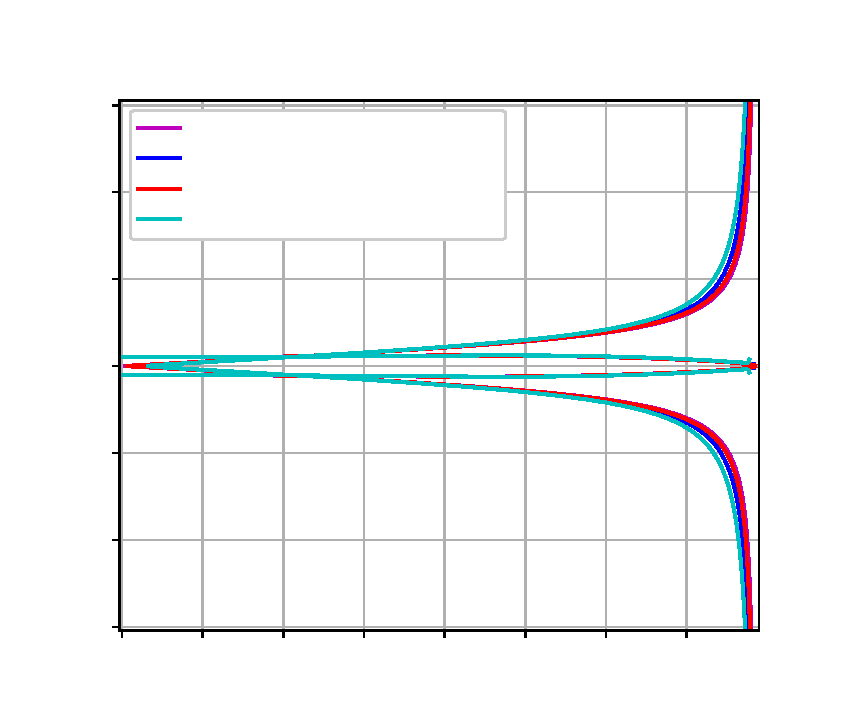
\includegraphics[width=\unitlength]{imagesbat/bat1p.eps}}%
    \put(0.10764293,0.05){\color[rgb]{0,0,0}\makebox(0,0)[lb]{\smash{0.0}}}%
    \put(0.20539672,0.05){\color[rgb]{0,0,0}\makebox(0,0)[lb]{\smash{0.2}}}%
    \put(0.30314899,0.05){\color[rgb]{0,0,0}\makebox(0,0)[lb]{\smash{0.4}}}%
    \put(0.40090404,0.05){\color[rgb]{0,0,0}\makebox(0,0)[lb]{\smash{0.6}}}%
    \put(0.49865657,0.05){\color[rgb]{0,0,0}\makebox(0,0)[lb]{\smash{0.8}}}%
    \put(0.59641162,0.05){\color[rgb]{0,0,0}\makebox(0,0)[lb]{\smash{1.0}}}%
    \put(0.69416414,0.05){\color[rgb]{0,0,0}\makebox(0,0)[lb]{\smash{1.2}}}%
    \put(0.79191667,0.05){\color[rgb]{0,0,0}\makebox(0,0)[lb]{\smash{1.4}}}%
    \put(0.05,0.08659355){\color[rgb]{0,0,0}\makebox(0,0)[lb]{\smash{-15}}}%
    \put(0.05,0.19199405){\color[rgb]{0,0,0}\makebox(0,0)[lb]{\smash{-10}}}%
    \put(0.07,0.29739355){\color[rgb]{0,0,0}\makebox(0,0)[lb]{\smash{-5}}}%
    \put(0.09,0.40279506){\color[rgb]{0,0,0}\makebox(0,0)[lb]{\smash{0}}}%
    \put(0.085,0.50819405){\color[rgb]{0,0,0}\makebox(0,0)[lb]{\smash{5}}}%
    \put(0.065,0.61359557){\color[rgb]{0,0,0}\makebox(0,0)[lb]{\smash{10}}}%
    \put(0.067,0.71899456){\color[rgb]{0,0,0}\makebox(0,0)[lb]{\smash{15}}}%
    \put(0.03065808,0.39910819){\color[rgb]{0,0,0}\rotatebox{90}{\makebox(0,0)[lb]{\smash{$\hat{\omega_0}$}}}}%
    \put(0.21843434,0.69249708){\color[rgb]{0,0,0}\makebox(0,0)[lb]{\smash{\footnotesize $R=1.0m, r_2=1cm$}}}%
    \put(0.21843434,0.65544658){\color[rgb]{0,0,0}\makebox(0,0)[lb]{\smash{\footnotesize$R=1.0m, r_2=5cm$}}}%
    \put(0.21843434,0.61839607){\color[rgb]{0,0,0}\makebox(0,0)[lb]{\smash{\footnotesize$R=0.5m, r_2=1cm $}}}%
    \put(0.21843434,0.58134557){\color[rgb]{0,0,0}\makebox(0,0)[lb]{\smash{\footnotesize$R=0.5m, r_2=5cm $}}}%
    \put(0.42,0.0){\color[rgb]{0,0,0}\makebox(0,0)[lb]{\smash{ $\theta_0 (rad)$}}}%
    \put(0.49865657,0.25){\color[rgb]{0,0,0}\makebox(0,0)[lb]{\smash{stable}}}%
    \put(0.49865657,0.5){\color[rgb]{0,0,0}\makebox(0,0)[lb]{\smash{stable}}}%
    \put(0.6,0.40279506){\color[rgb]{0,0,0}\makebox(0,0)[lb]{\smash{instable}}}%
  \end{picture}%
\endgroup%

\def\svgwidth{250}
%% Creator: Inkscape inkscape 0.92.2, www.inkscape.org
%% PDF/EPS/PS + LaTeX output extension by Johan Engelen, 2010
%% Accompanies image file 'bat2p.eps' (pdf, eps, ps)
%%
%% To include the image in your LaTeX document, write
%%   \input{<filename>.pdf_tex}
%%  instead of
%%   \includegraphics{<filename>.pdf}
%% To scale the image, write
%%   \def\svgwidth{<desired width>}
%%   \input{<filename>.pdf_tex}
%%  instead of
%%   \includegraphics[width=<desired width>]{<filename>.pdf}
%%
%% Images with a different path to the parent latex file can
%% be accessed with the `import' package (which may need to be
%% installed) using
%%   \usepackage{import}
%% in the preamble, and then including the image with
%%   \import{<path to file>}{<filename>.pdf_tex}
%% Alternatively, one can specify
%%   \graphicspath{{<path to file>/}}
%% 
%% For more information, please see info/svg-inkscape on CTAN:
%%   http://tug.ctan.org/tex-archive/info/svg-inkscape
%%
\begingroup%
  \makeatletter%
  \providecommand\color[2][]{%
    \errmessage{(Inkscape) Color is used for the text in Inkscape, but the package 'color.sty' is not loaded}%
    \renewcommand\color[2][]{}%
  }%
  \providecommand\transparent[1]{%
    \errmessage{(Inkscape) Transparency is used (non-zero) for the text in Inkscape, but the package 'transparent.sty' is not loaded}%
    \renewcommand\transparent[1]{}%
  }%
  \providecommand\rotatebox[2]{#2}%
  \ifx\svgwidth\undefined%
    \setlength{\unitlength}{395.9999901bp}%
    \ifx\svgscale\undefined%
      \relax%
    \else%
      \setlength{\unitlength}{\unitlength * \real{\svgscale}}%
    \fi%
  \else%
    \setlength{\unitlength}{\svgwidth}%
  \fi%
  \global\let\svgwidth\undefined%
  \global\let\svgscale\undefined%
  \makeatother%
  \begin{picture}(1,0.833939)%
    \put(0,0){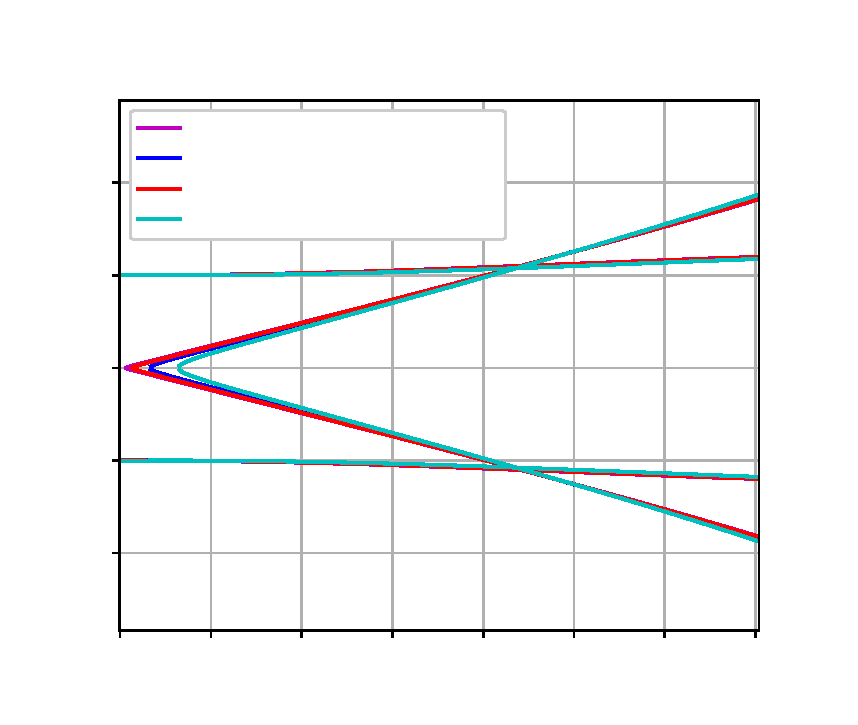
\includegraphics[width=\unitlength]{imagesbat/bat2p.eps}}%
    \put(0.10533056,0.05){\color[rgb]{0,0,0}\makebox(0,0)[lb]{\smash{0.0}}}%
    \put(0.21535177,0.05){\color[rgb]{0,0,0}\makebox(0,0)[lb]{\smash{0.1}}}%
    \put(0.32537374,0.05){\color[rgb]{0,0,0}\makebox(0,0)[lb]{\smash{0.2}}}%
    \put(0.43539394,0.05){\color[rgb]{0,0,0}\makebox(0,0)[lb]{\smash{0.3}}}%
    \put(0.54541414,0.05){\color[rgb]{0,0,0}\makebox(0,0)[lb]{\smash{0.4}}}%
    \put(0.65543434,0.05){\color[rgb]{0,0,0}\makebox(0,0)[lb]{\smash{0.5}}}%
    \put(0.76545707,0.05){\color[rgb]{0,0,0}\makebox(0,0)[lb]{\smash{0.6}}}%
    \put(0.87547727,0.05){\color[rgb]{0,0,0}\makebox(0,0)[lb]{\smash{0.7}}}%
    \put(0.035,0.17609683){\color[rgb]{0,0,0}\makebox(0,0)[lb]{\smash{-1.0}}}%
    \put(0.04,0.28830516){\color[rgb]{0,0,0}\makebox(0,0)[lb]{\smash{-0.5}}}%
    \put(0.05,0.40051223){\color[rgb]{0,0,0}\makebox(0,0)[lb]{\smash{0.0}}}%
    \put(0.05,0.5127193){\color[rgb]{0,0,0}\makebox(0,0)[lb]{\smash{0.5}}}%
    \put(0.05,0.62492637){\color[rgb]{0,0,0}\makebox(0,0)[lb]{\smash{1.0}}}%
    \put(0.03065808,0.39910819){\color[rgb]{0,0,0}\rotatebox{90}{\makebox(0,0)[lb]{\smash{$\hat{\omega_0}$}}}}%
    \put(0.21843434,0.69249708){\color[rgb]{0,0,0}\makebox(0,0)[lb]{\smash{\footnotesize $R=1.0m, r_2=1cm$}}}%
    \put(0.21843434,0.65544658){\color[rgb]{0,0,0}\makebox(0,0)[lb]{\smash{\footnotesize$R=1.0m, r_2=5cm$}}}%
    \put(0.21843434,0.61839607){\color[rgb]{0,0,0}\makebox(0,0)[lb]{\smash{\footnotesize$R=0.5m, r_2=1cm $}}}%
    \put(0.21843434,0.58134557){\color[rgb]{0,0,0}\makebox(0,0)[lb]{\smash{\footnotesize$R=0.5m, r_2=5cm $}}}%
    \put(0.42,0.0){\color[rgb]{0,0,0}\makebox(0,0)[lb]{\smash{ $\theta_0 (rad)$}}}%
    \put(0.35,0.18609683){\color[rgb]{0,0,0}\makebox(0,0)[lb]{\smash{\footnotesize stable}}}%
    \put(0.65543434,0.40051223){\color[rgb]{0,0,0}\makebox(0,0)[lb]{\smash{\footnotesize instable}}}%
    \put(0.13,0.34){\color[rgb]{0,0,0}\makebox(0,0)[lb]{\smash{\footnotesize instable en}}}%
    \put(0.13,0.31){\color[rgb]{0,0,0}\makebox(0,0)[lb]{\smash{\footnotesize cas de perturbation}}}%
  \end{picture}%
\endgroup%

\caption{Carte de stabilité. Les frontières déterminent l'existence d'une position d'équilibre dynamique pour chaque couple ($\theta_0,\hat{\omega_0}$), où $\hat{\omega_0}$ correspond à la vitesse de rotation adimensionnelle, $\hat{\omega_0}=\omega_0 \sqrt{\dfrac{R+r_2}{g}}$}
\end{figure}

